\documentclass[10 pt]{article}

\usepackage{graphicx}

\begin{document}

\begin{figure}[htbp]
\begin{center}
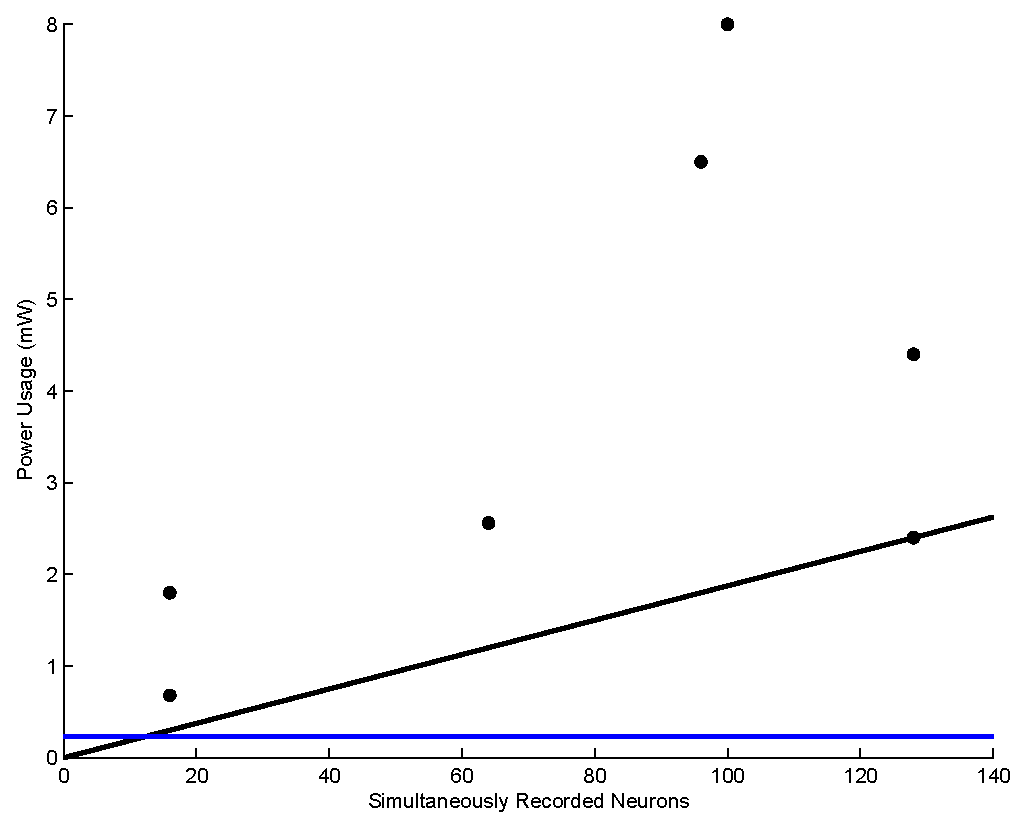
\includegraphics[scale=0.30]{power.eps}
\caption{Power usage for simultaneously recording neurons. The black line represents the best power usage of 0.019 mW / neuron achieved by \cite{???}. The blue line indicates the total power usage of 0.23 mW allowed to support the Medtroic Model 37601 Activa PC neurostimulator battery for 10 years. Using current technology, only approximately 12 neurons can be simultaneously sampled.}
\label{fig:power}
\end{center}
\end{figure}

\begin{figure}[htbp]
\begin{center}
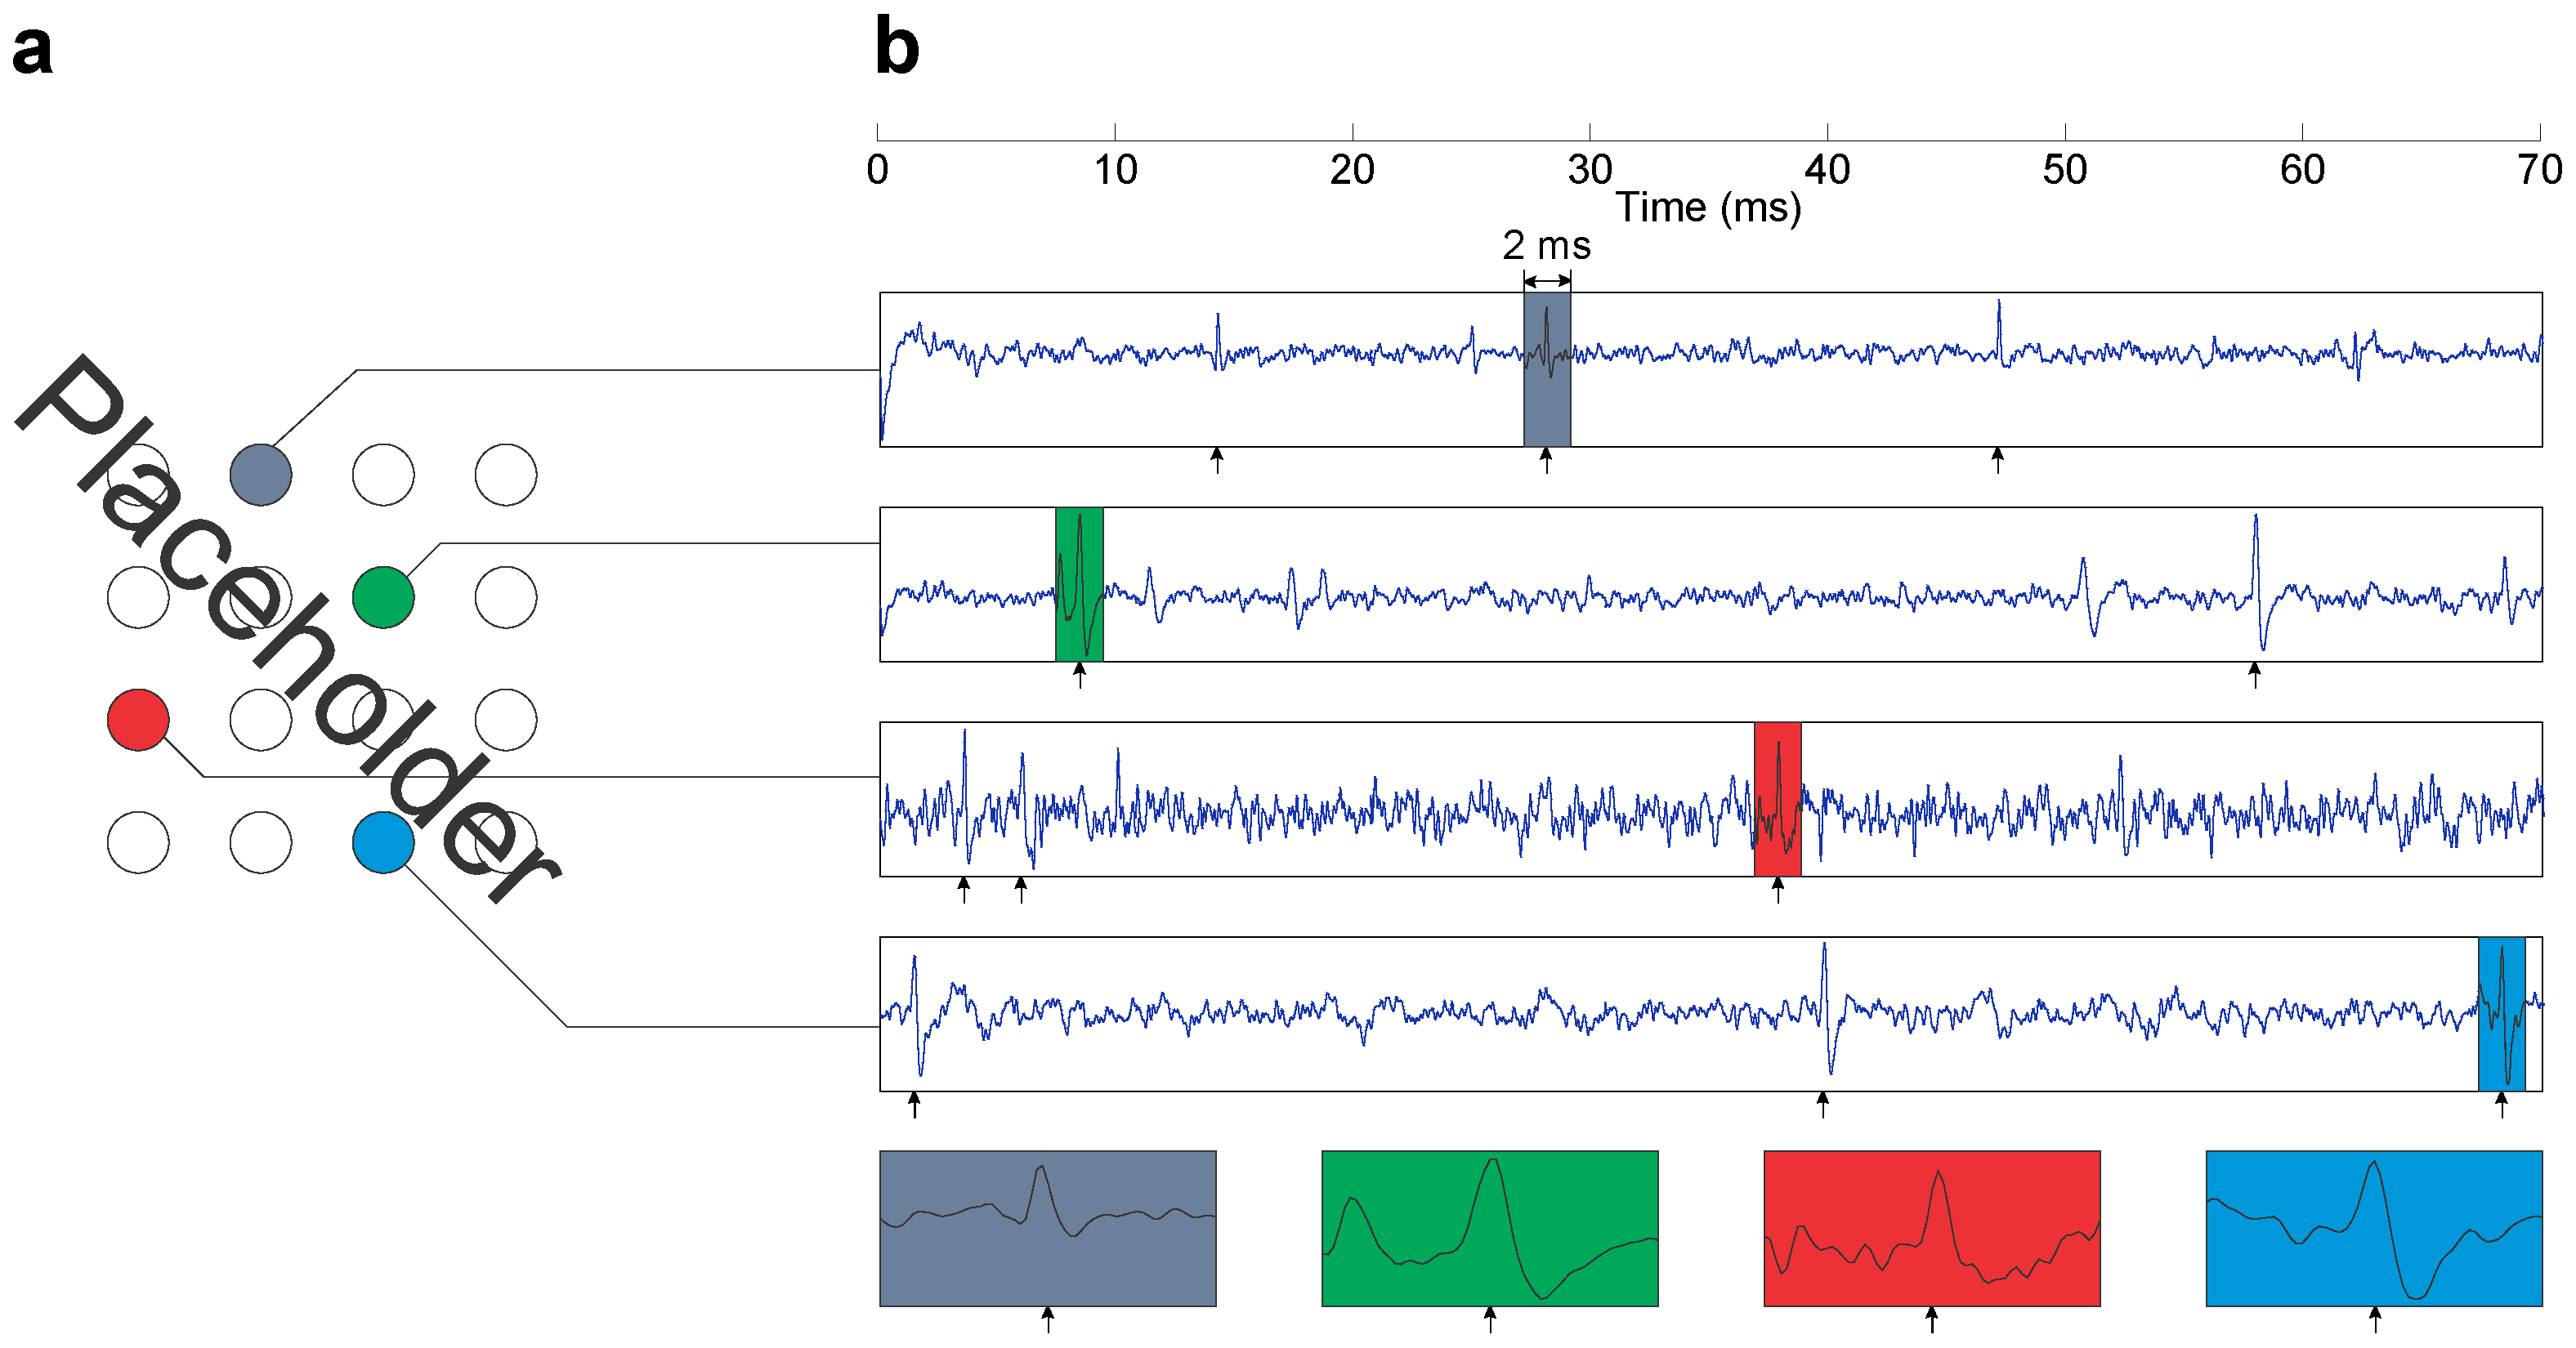
\includegraphics[scale=0.22]{sample.eps}
\caption{Electrode positions and sample neuron spikes. (\textbf{a}) A 16-electrode ``floating'' microelectrode array placed in the brain. (\textbf{b}) Voltage traces for four sample electrodes. Spikes detected by commercial software \cite{???} are indicated by arrows. The electodes each are recording spikes from one neuron, and each neuron has a characteristic spike shape.} % Name of commercial software ???
\label{fig:sample}
\end{center}
\end{figure}

\begin{figure}[htbp]
\begin{center}
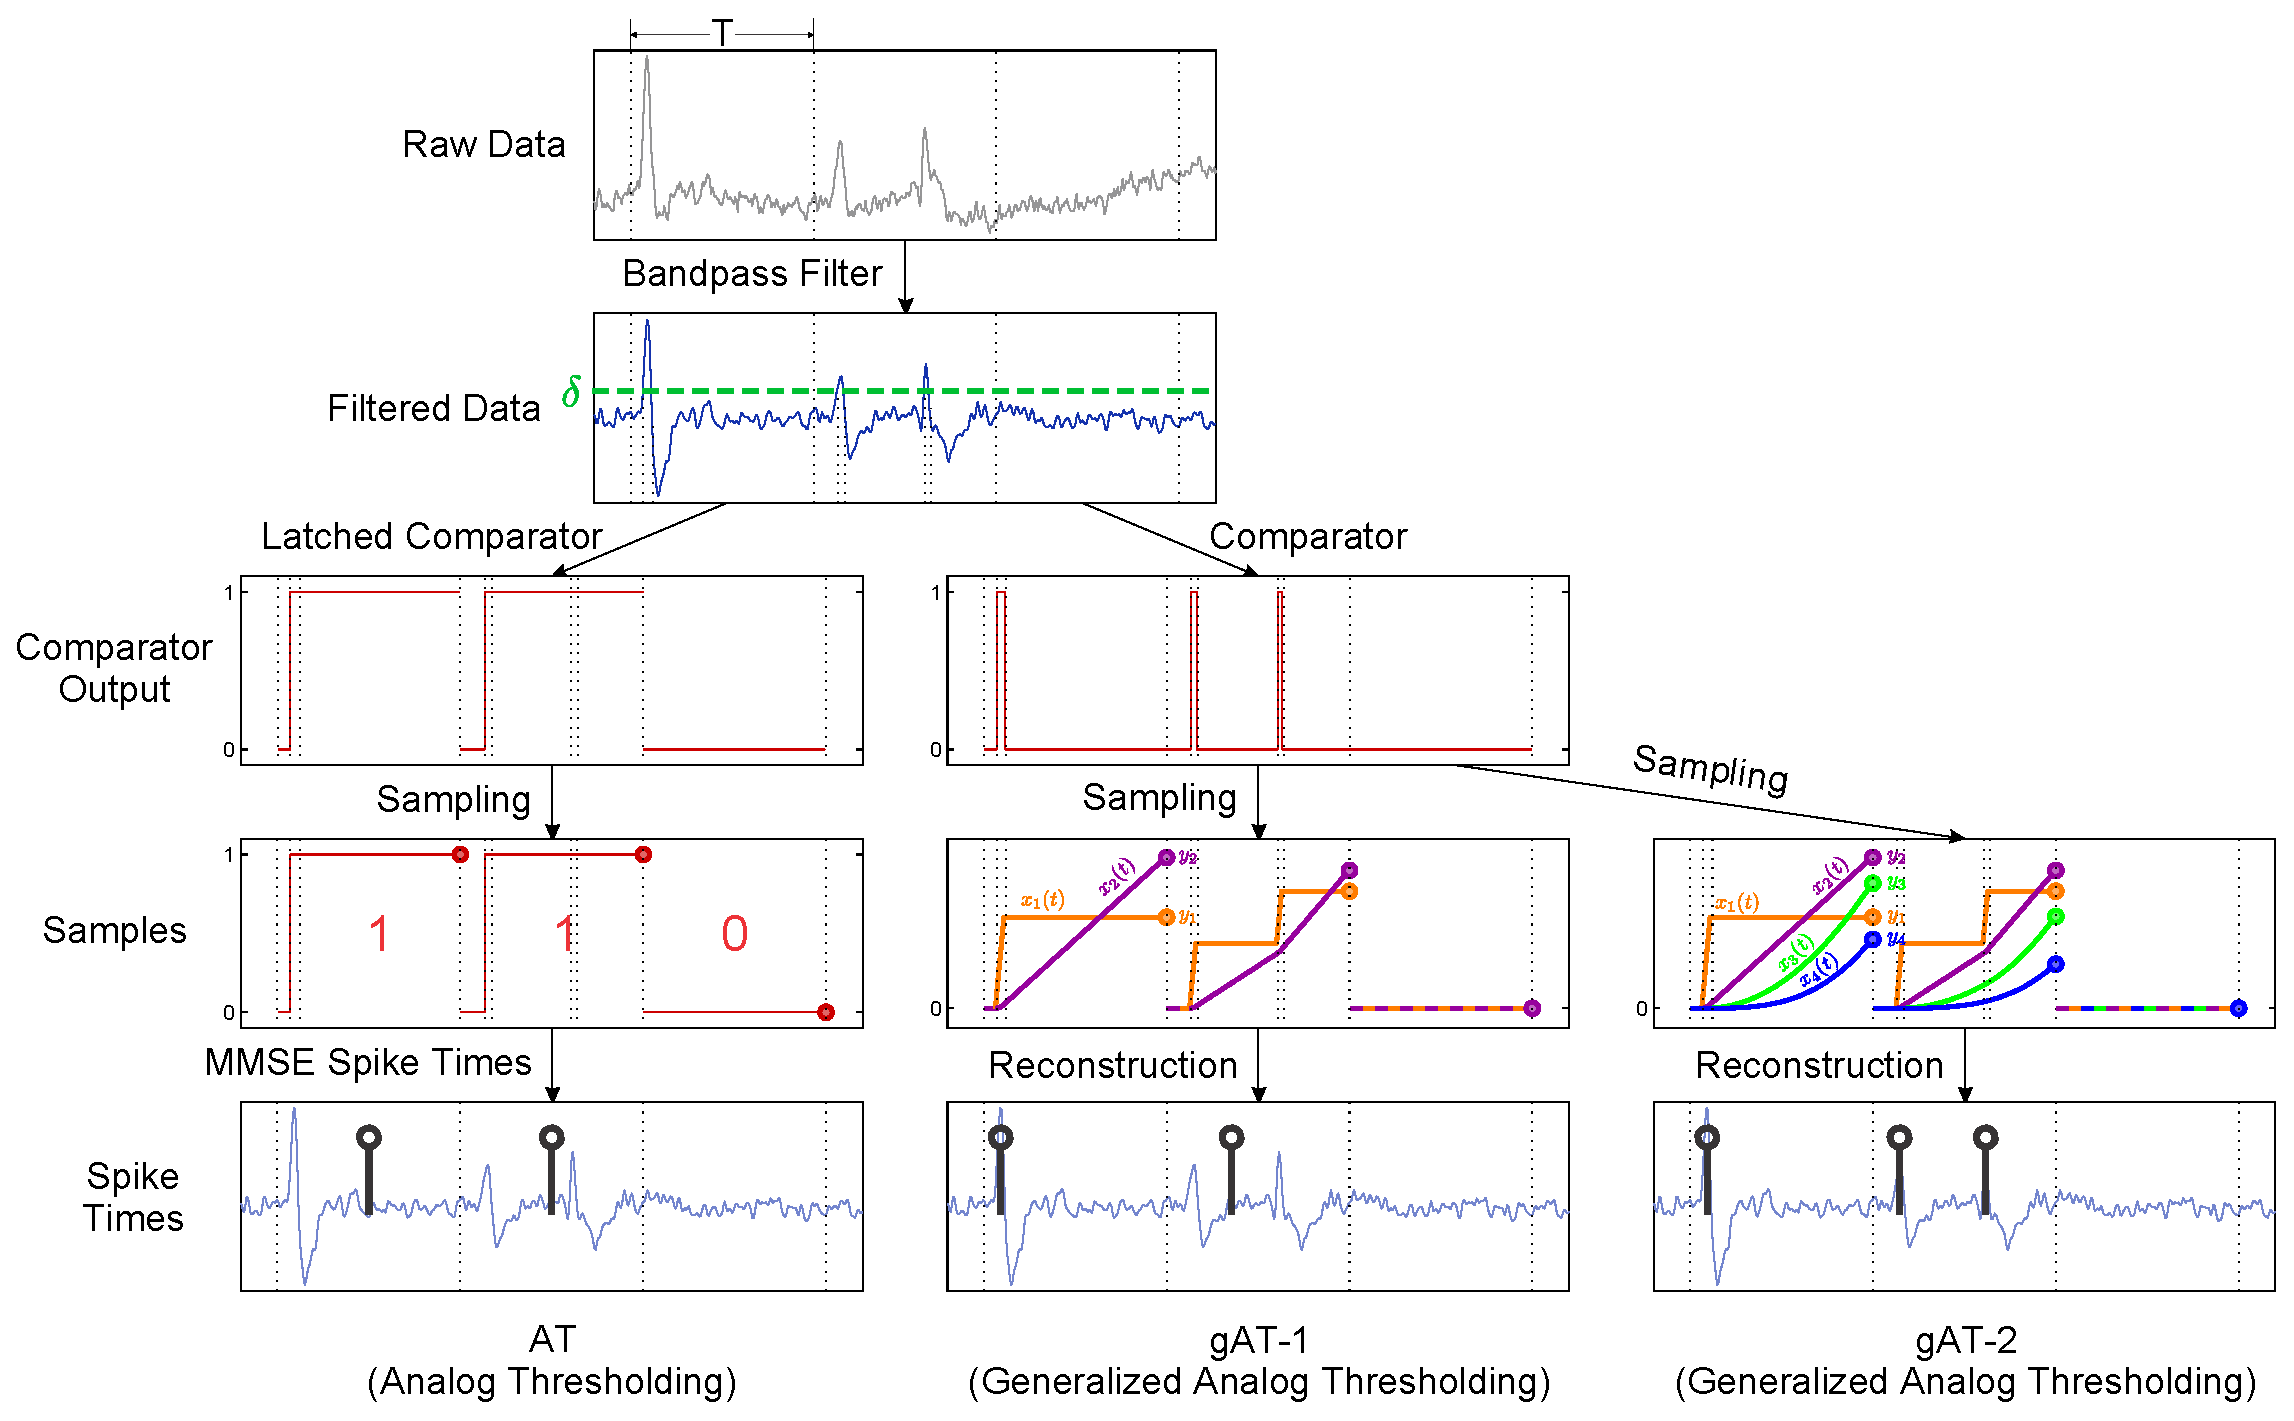
\includegraphics[scale=0.30]{at_gat.eps}
\caption{Comparison of analog thresholding (AT) and generalized analog thresholding (gAT-1 and gAT-2). Using commercial software, one spike was detected in the first sampling period, two spikes were detected in the second sampling period, and no spikes were detected in the third sampling period. All three methods are able to correctly identify when no spikes are present and when a single spike is present; however, analog thresholding provides no information about the position of the spike, so the spike is simply reported to be in the center of the interval. Only gAT-2 is able to identify two spikes correctly.} % Name of the commercial software ???
\label{fig:at_gat}
\end{center}
\end{figure}

\begin{figure}[htbp]
\begin{center}
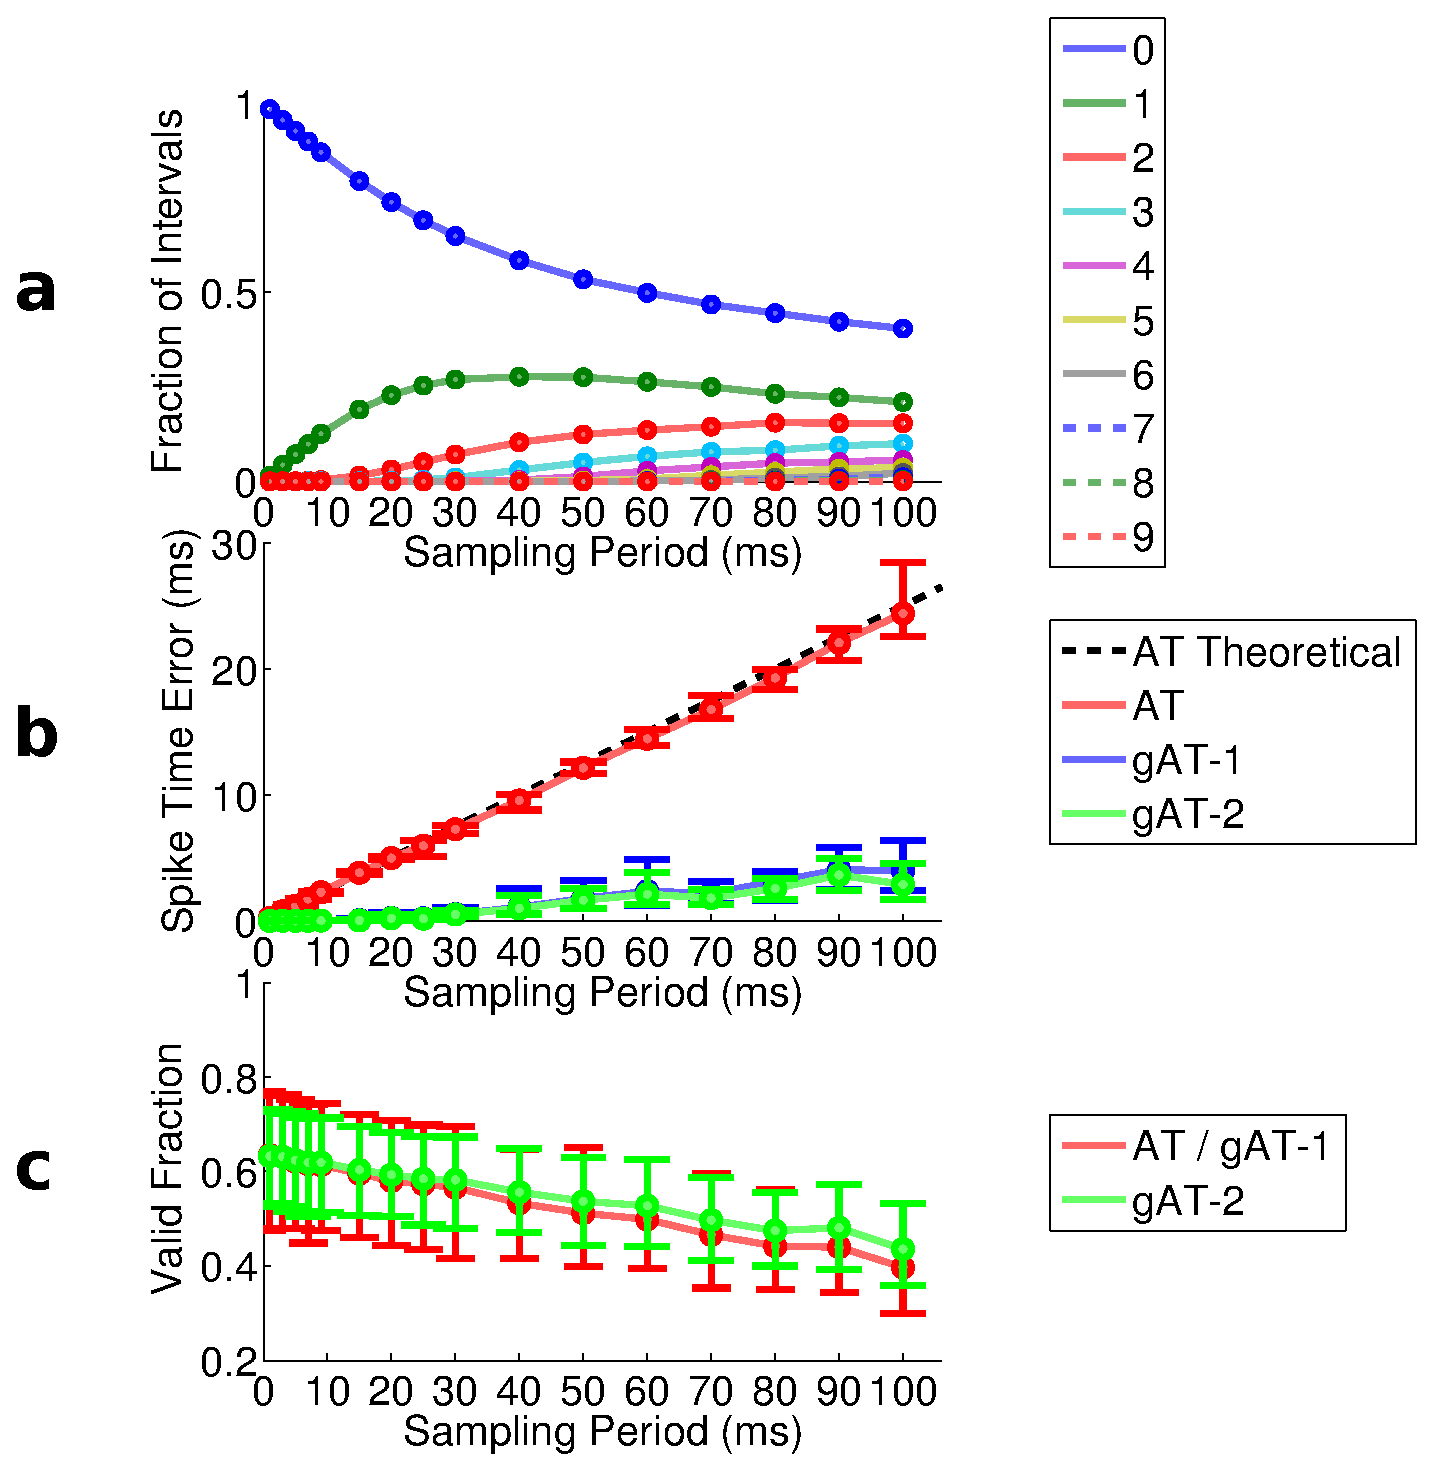
\includegraphics[scale=0.35]{basic_comparison.eps}
\caption{Basic comparison of the sampling methods at different sampling periods. (\textbf{a}) The fraction of intervals with a certain number of spikes within the interval. As the sampling period increases, intervals tend to have larger numbers of spikes. (\textbf{b}) Average error in estimated spike time in intervals with exactly one correctly identified spike. AT always predicts that the spike is at the center of the interval, and its behavior closely matches the theoretical curve. gAT-1 and gAT-2 have much lower errors than AT. (\textbf{c}) The fraction of intervals that correctly identify the number of spikes. AT and gAT-1 always predict the same number of spikes because they are only able to differentiate between intervals with no spikes and intervals with a non-zero number of spikes. gAT-2 is able to differentiate between intervals with one spike and intervals with two spikes, and gAT-2 is able to improve the accuracy of spike count predictions.}
\label{fig:basic_comparison}
\end{center}
\end{figure}

\begin{figure}[htbp]
\begin{center}
\includegraphics[scale=0.30]{roc.eps}
\caption{Tradeoff between false positives and false negatives. False positives are defined as predicted spikes without a corresponding real spike, and false negatives are defines as real spikes without a corresponding predicted spike. An error tolerance of $\tau = 5\textrm{ ms}$ is allowed. Each point corresponds to a different spike detection threshold $\delta$. Increasing $\delta$ lowers the number of false positives but increases the number of false negatives. The large data point on each curve shows the optimal $\delta$, which is the point with the fewest possible total errors. Three representative curves (worst, median, and best) are shown for each method. gAT-2 has the best performance and AT has the worst performance. As the sampling period increases, all three methods perform worse.} % refractory period ???
\label{fig:ROC}
\end{center}
\end{figure}

\begin{figure}[htbp]
\begin{center}
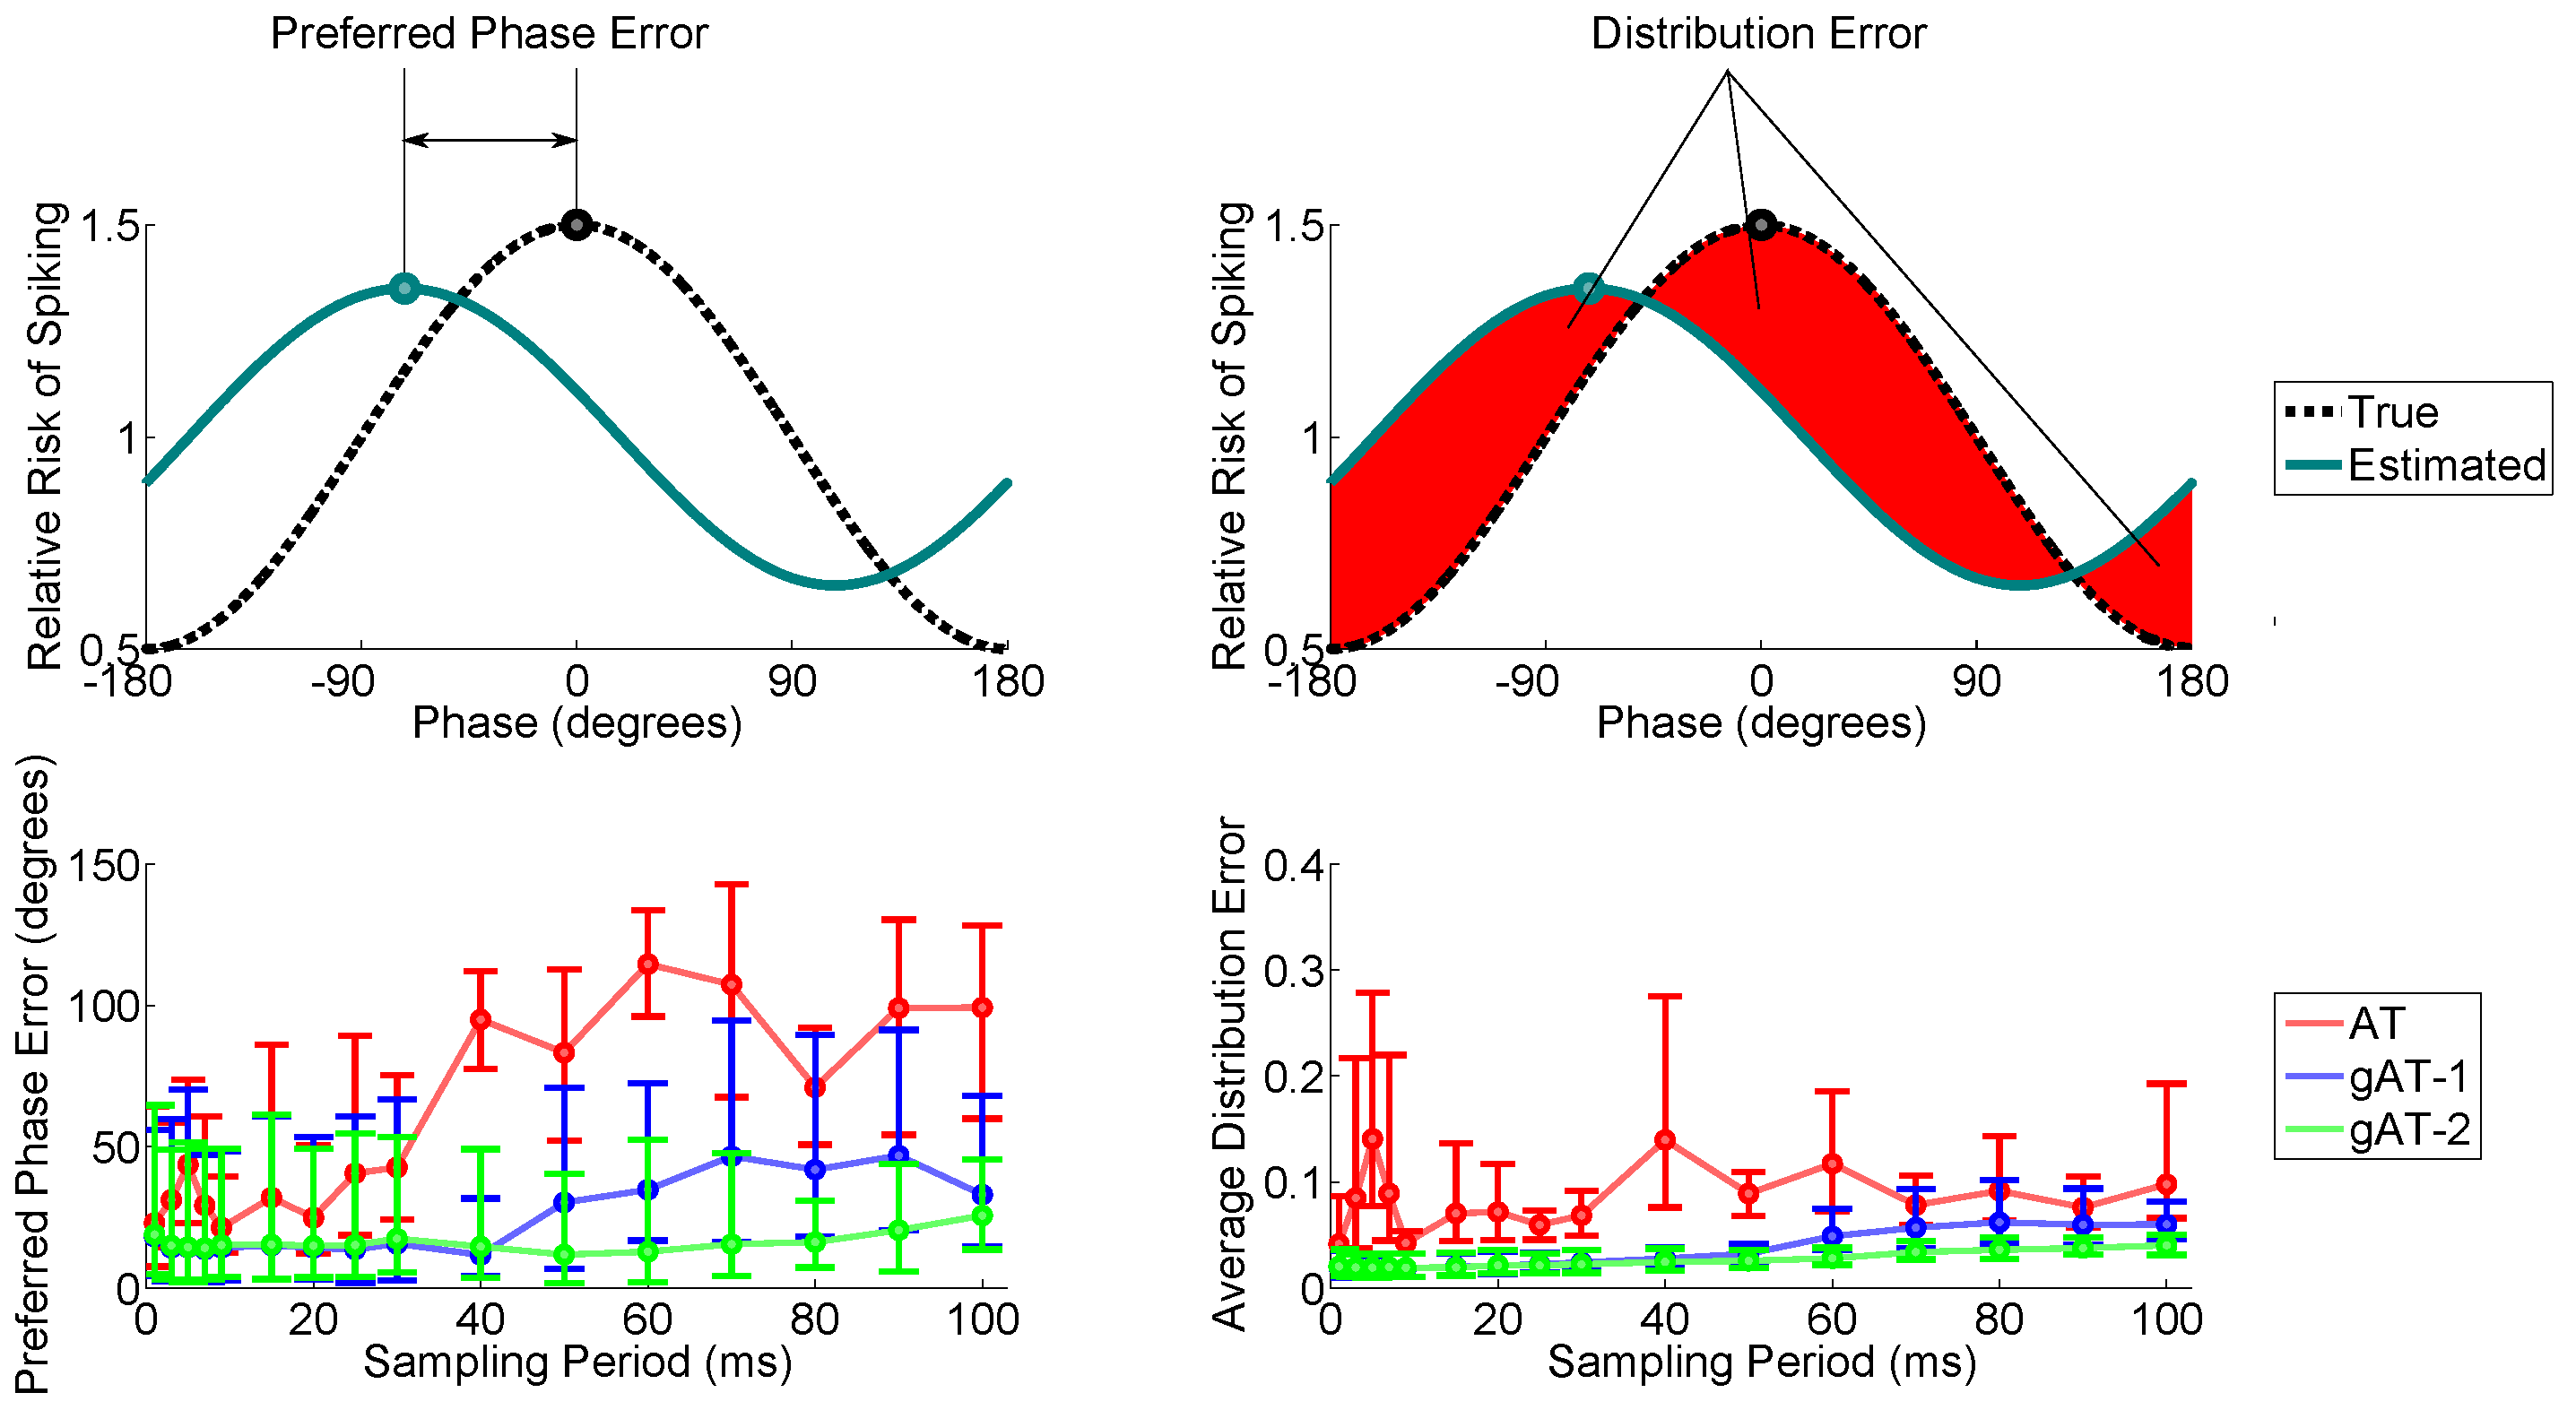
\includegraphics[scale=0.30]{LFP_error.eps}
\caption{Error of the local field potential phase locking. (\textbf{a}) Explanation of preferred phase error (difference between the maxima of the two curves). (\textbf{b}) Explanation of distribution error (area between true curve and predicted curve). (\textbf{c}) Preferred phase error for different sampling periods. (\textbf{d}) Distribution error for different sampling periods.}
\label{fig:LFP_error}
\end{center}
\end{figure}

\begin{figure}[htbp]
\begin{center}
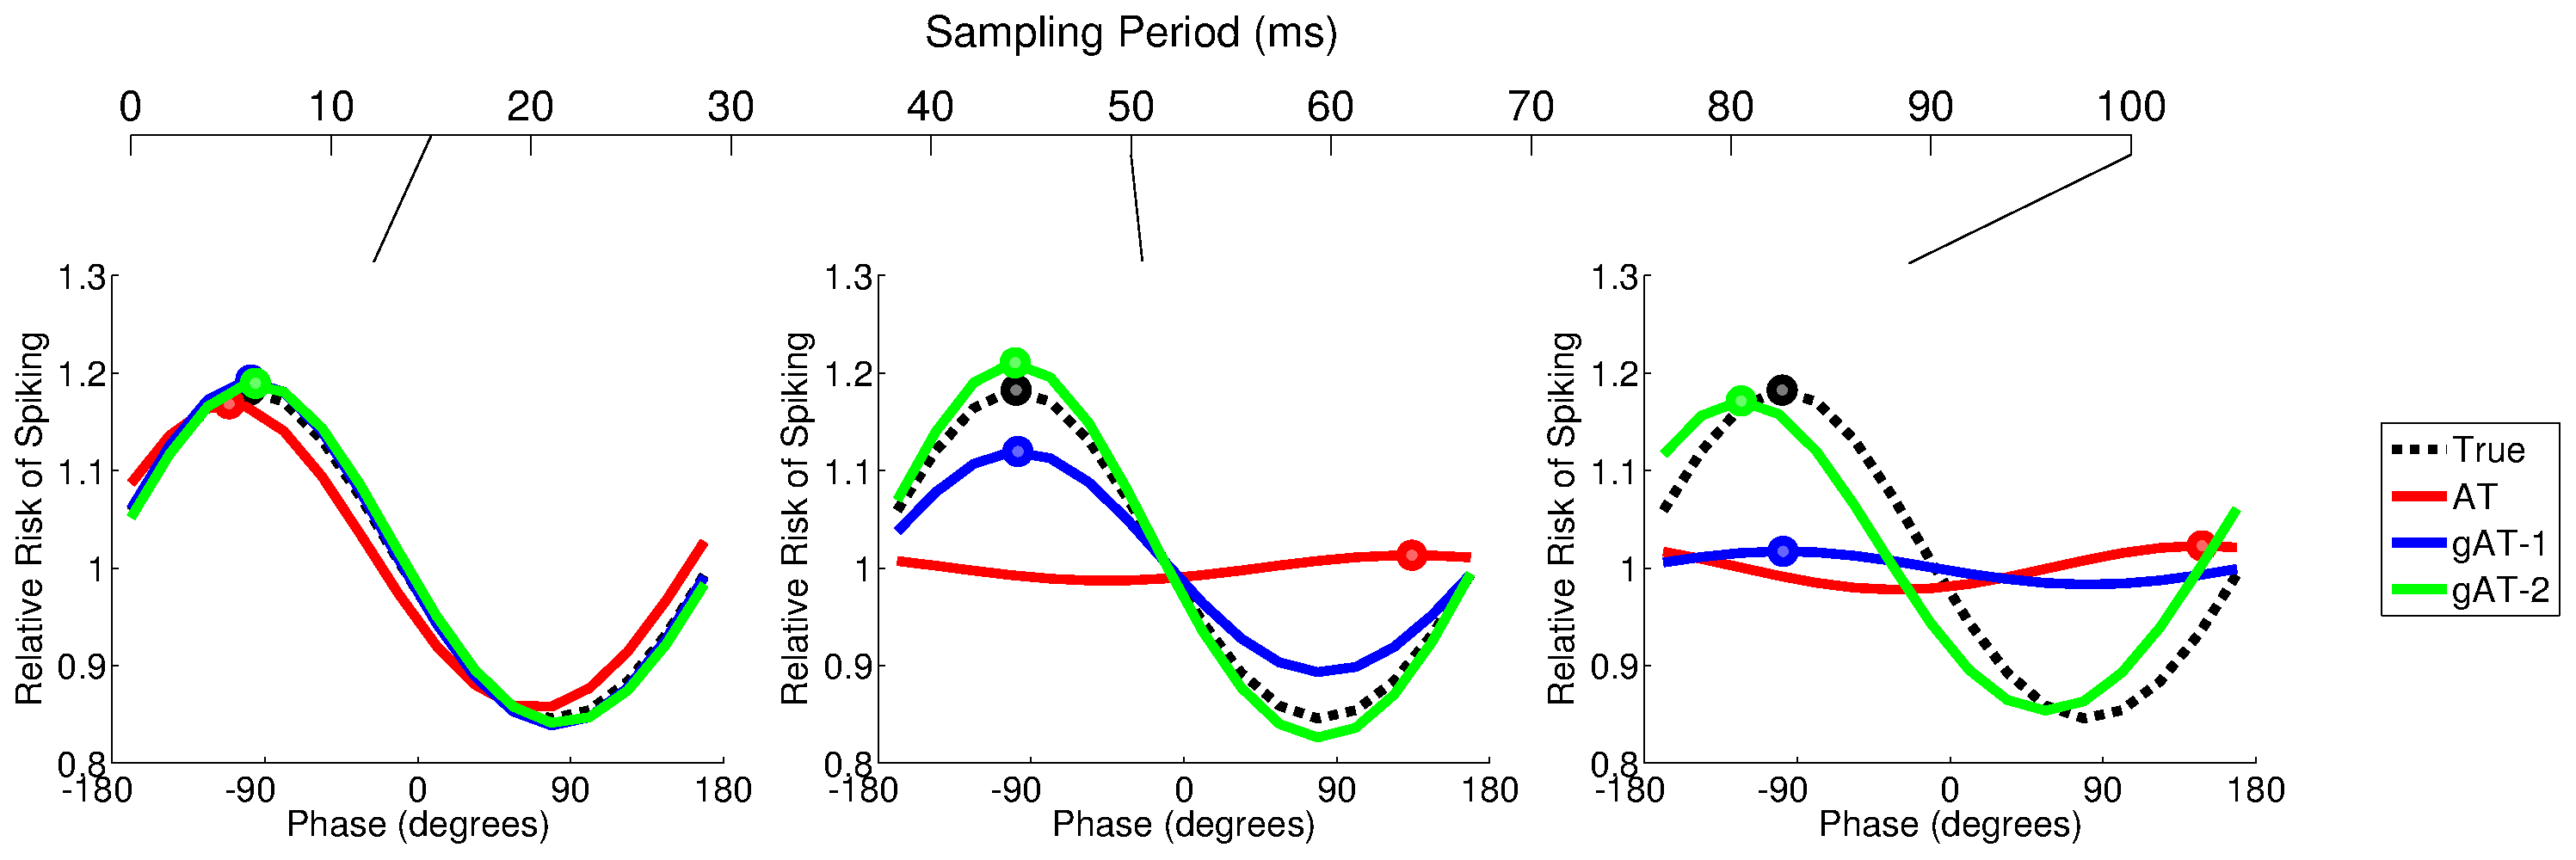
\includegraphics[scale=0.30]{LFP.eps}
\caption{Local field potential phase locking. For short sampling periods, all three methods perform well, but as the sampling period increases, AT begins to decay in performance first, and gAT-1 decays in performance next.}
\label{fig:LFP}
\end{center}
\end{figure}

\begin{figure}[htbp]
\begin{center}
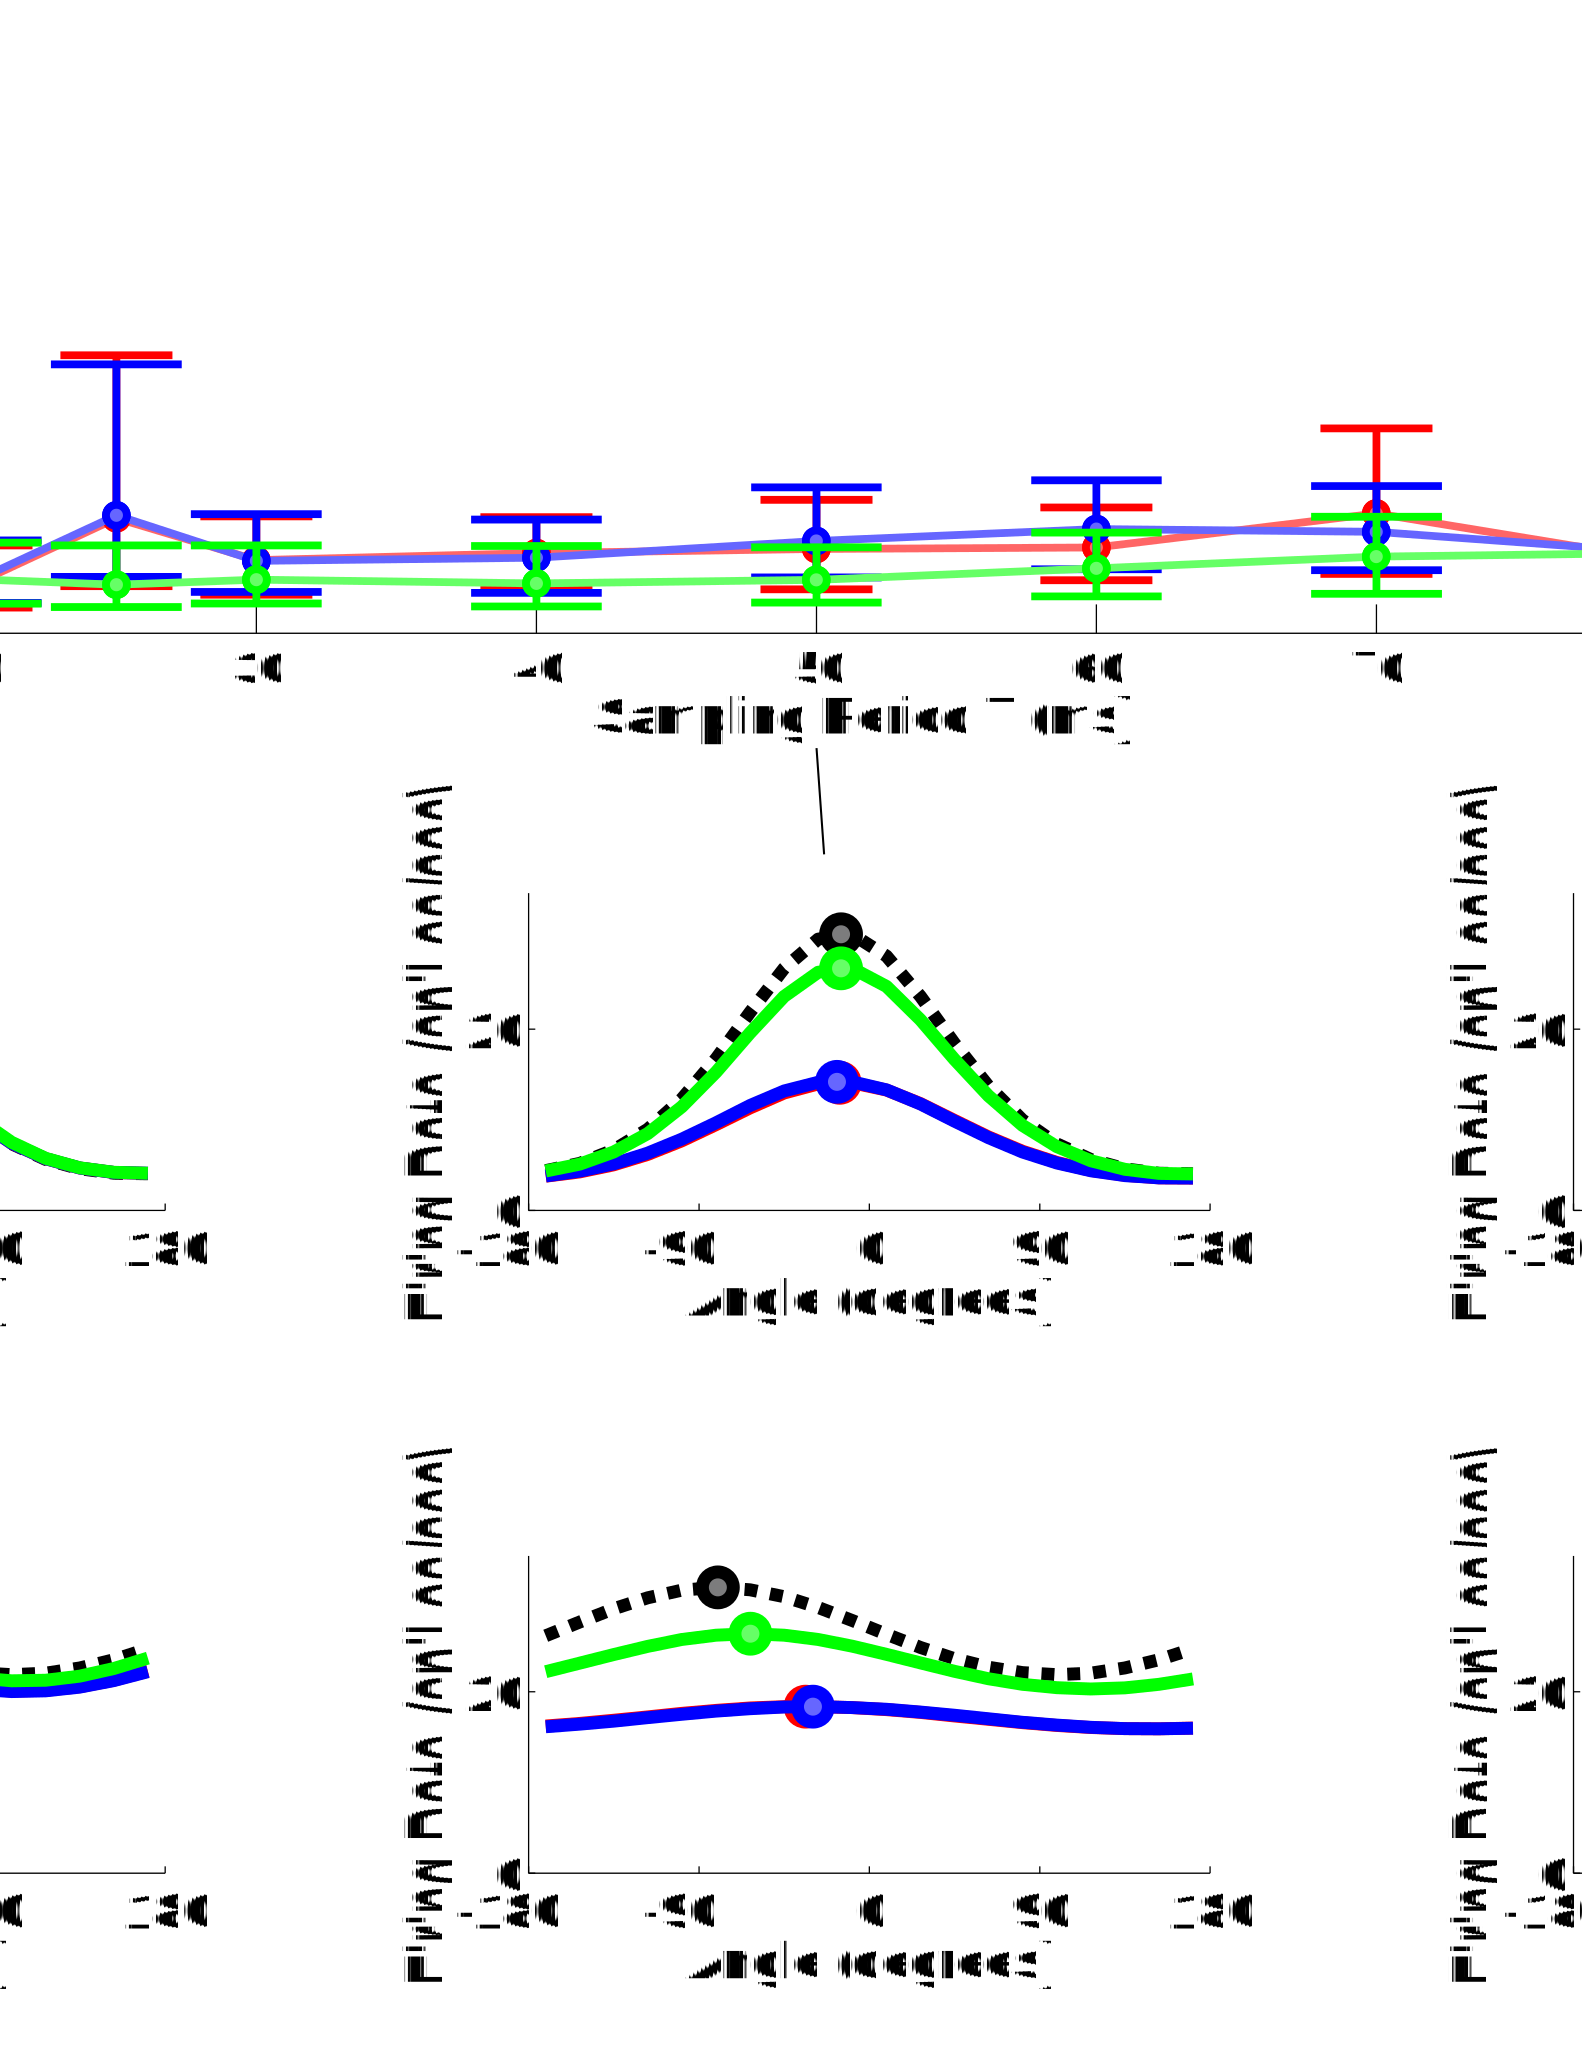
\includegraphics[scale=0.30]{saturation.eps}
\label{fig:saturation}
\caption{Tuning curve errors and saturation effect. The error for gAT-2 is the lowest of the three methods. The two neurons shown have similar maximum spiking rates, but the minimum spiking rate is higher for the second neuron. As a result, the preferred direction is predicted more accurately for the first neuron.}
\end{center}
\end{figure}

\end{document}

